\RequirePackage[T1]{fontenc}
\documentclass[conference]{IEEEtran}
\usepackage{amsmath,amssymb,booktabs,graphicx,url}
\usepackage[hidelinks]{hyperref}
\setlength{\dblfloatsep}{8pt}
\setlength{\dbltextfloatsep}{12pt}
\graphicspath{{../results/connectivity_experiment/analysis_v2/}}
% Generated from frozen connectivity statistics. Do not edit numbers manually.
\newcommand{\FullStd}{96.6}
\newcommand{\ArrivalStd}{96.9}
\newcommand{\SuccessDeltaStd}{-0.3}
\newcommand{\SuccessLowStd}{-2.6}
\newcommand{\SuccessHighStd}{2.0}
\newcommand{\CostChangeStd}{-24.5}
\newcommand{\DelayChangeStd}{186.7}
\newcommand{\HandoverChangeStd}{-95.5}
\newcommand{\FullFailuresStd}{34}
\newcommand{\CommonStd}{945}
\newcommand{\FullLong}{89.7}
\newcommand{\ArrivalLong}{86.3}
\newcommand{\SuccessDeltaLong}{3.4}
\newcommand{\SuccessLowLong}{-1.0}
\newcommand{\SuccessHighLong}{8.1}
\newcommand{\CostChangeLong}{-14.7}
\newcommand{\DelayChangeLong}{261.1}
\newcommand{\HandoverChangeLong}{-92.8}
\newcommand{\FullFailuresLong}{103}
\newcommand{\CommonLong}{802}

\title{Restoring Connectivity Constraints in Joint UAV Trajectory and Handover Control}
\author{\IEEEauthorblockN{Guillem Moreno Garcia and Evgenii Vinogradov}
\IEEEauthorblockA{Universitat Polit\`ecnica de Catalunya, Barcelona, Spain\\Research draft, 12 September 2026}}
\begin{document}
\maketitle
\begin{abstract}
Restoring destination arrival does not establish that a cellular UAV maintains
its required connection. We audit an earlier reward repair and implement a
separate study with strict sampled received signal strength and buffer
constraints, together with the original thesis's delay, interference and
handover objectives. A received Barcelona radio map supplies the channel data.
All new controllers share explicit surrogate dynamics and a prospective safety
filter; learned controllers add bounded motion corrections to a braking
reference and select among available station/resource actions. Two reward arms
use five training seeds and fresh standard and longer route sets. Joint mission
success is \FullStd\% and \FullLong\% with the full radio cost, versus
\ArrivalStd\% and \ArrivalLong\% without that cost. On paired successful
standard flights, accumulated radio cost changes by \CostChangeStd\%, while
the mean delay proxy changes by \DelayChangeStd\%. Four deterministic
references expose the contributions and limits of network control and local
route planning. Every reported successful flight satisfies the sampled RSS and
buffer constraints. This repairs the objective and endpoint within the declared
surrogate; it does not establish continuous physical connectivity, improvement
in every communication metric, or reproduction of the original simulator.
\end{abstract}
\begin{IEEEkeywords}
Cellular UAV, connectivity constraints, handover, trajectory control, reward
design, reinforcement learning, reproducibility.
\end{IEEEkeywords}

\section{Introduction}
A master's thesis considers joint trajectory and handover control using a
Barcelona ray tracing environment~\cite[pp.~6--7, Sec.~3.1]{thesis}. Its objective
combines delay, interference and handovers~\cite[p.~10, Eq.~(11)]{thesis}, while
its constraints require minimum serving RSS and bounded queue occupancy
\cite[p.~11, Eq.~(12), C2 and C4]{thesis}. The source nevertheless reports
wandering and prioritization of connectivity over destination completion
\cite[p.~19, Sec.~7.2; p.~21, Sec.~8]{thesis}.

An earlier controlled reimplementation replaced a binary approach reward and
restored arrival on the received map. That finding had a narrower scope than
the full joint task: mission success permitted brief RSS outages, communication
feasibility was partly a subsequent label, and the replacement reward omitted
direct interference cost. A follow up audit motivated the present study.

We correct the sampled joint endpoint and objective through a controlled
comparison with retained development failures. The original simulator remains
unavailable. Citations give printed thesis pages; add two for the PDF viewer
page. Accompanying Markdown notes contain complete implementation comparisons.

\section{Source Requirements and Audit}
\subsection{Which Communication Requirements Apply?}
We use the thesis requirements, not a newly imposed application service level.
The RSS minimum is $-96$ dBm and the buffer is listed as 160 KB
\cite[p.~15, Table~3]{thesis}; we retain the explicit 1,280,000 bit interpretation.
The written C2 inequality allows equality and applies at every modeled time
\cite[p.~11, Eq.~(12)]{thesis}. Delay remains an optimized quantity, defined in
the source as queue divided by service rate~\cite[p.~9, Eq.~(4)]{thesis}.
Neither a two second packet deadline nor an empty queue arrival condition is
introduced. A successful arrival can therefore retain queued data; it must not
be described as completed data delivery.

The distinction between formulation and enforcement matters. The source reward
penalizes RSS violations~\cite[p.~12, Eq.~(14)]{thesis}, which does not establish
that its unavailable implementation guaranteed C2. Its direct data dump penalty
was removed during development~\cite[pp.~20--21, Sec.~7.3]{thesis}. We compare
verified written definitions with our executable rules, not inferred behavior
of missing original code.

\subsection{Why the Earlier Arrival Result Was Insufficient}
The original map audit found at least 38 operator 1 stations strictly above
$-96$ dBm at every grid location. The strongest station ranges from $-51$ to
$-25$ dBm. Consequently, an RSS coverage hole does not force a detour if any
suitable station could be selected. Actual association constraints and
interference still matter.

An exact replay of 4,400 earlier flights added service diagnostics without
changing their saved outcomes. In the earlier reward replacement's 1,000
standard evaluations, arrival was 100\%, but only 92.2\% had no sampled RSS
outage. Modeled capacity was below the 200 kbit/s offered rate for a mean
26.6\% of each flight, and 20.2\% arrived with a nonempty queue. A transient
capacity deficit is not itself disconnection because buffering can absorb it.
These measures expose what the old endpoint did and did not establish; they
are not a new confirmatory policy comparison.

\section{Revised Surrogate and Controller}
\subsection{Shared Physical Assumptions}
We preserve the received native resolution RSS map, selecting the first
operator's 87 stations. Matching source metadata includes 2.1 GHz and 100 m
altitude~\cite[p.~7, Table~2; p.~15, Table~3]{thesis}; this does not prove an
identical original dataset version. The raw private HDF5 is not modified or
published. The provisional $-128$ sentinel interpretation remains unverified.

The shared model retains a one second decision step, acceleration norm limit
5 m/s$^2$, speed limit 25 m/s, 200 s deadline, and a 100 kJ budget under the
engineering energy proxy $100+0.4v^2$ watts. These are the earlier surrogate's
settings. They differ from the source's 0.1 s table step and 100 m/s speed
setting~\cite[p.~15, Table~3]{thesis}; the source also gives a conflicting
1 ms interval in prose~\cite[p.~14, Sec.~6.1]{thesis}.

The radio proxy retains 12 resource groups, half occupied by a deterministic
station pattern. Interference sums linear received power from cochannel
background stations. Capacity is $1.44\cdot10^6\log_2(1+\mathrm{SINR})$ bit/s,
with noise $-103.41$ dBm and offered traffic 200,000 bit/s. The source's printed
rate and SNR expressions differ~\cite[p.~10, Eqs.~(7)--(8)]{thesis}, and its
background occupancy is described as random~\cite[p.~14, Sec.~6.1]{thesis}.
We retain these declared surrogate assumptions to separate the current repair
from a new propagation or traffic model. The interference is a downlink proxy,
not a calibrated uplink quantity matching the source's terminology
\cite[p.~10, Eq.~(9)]{thesis}.

\subsection{Joint Success and Failure}
Let $d_t$ denote destination distance and $q_t$ the queue after the sampled
arrival/service update. Joint success requires arrival by the deadline with
$d_T\leq10$ m and $\|v_T\|\leq2$ m/s, together with
\begin{equation}
\mathrm{RSS}_{k_t}(p_t)\geq-96\ \mathrm{dBm},\quad
0\leq q_t\leq1{,}280{,}000\ \mathrm{bits},\quad\forall t.
\end{equation}
The 10 m tolerance follows the source table~\cite[p.~15, Table~3]{thesis}; the
numeric stopping tolerance is our explicit interpretation of stopping at the
destination~\cite[p.~9, Sec.~3.2]{thesis}. Map and energy conditions also apply.
A single sampled RSS violation or any buffer overflow ends a failed mission.
Failure takes precedence over simultaneous arrival. Initial RSS is checked;
queue clipping for storage cannot erase an overflow flag.

This enforces the constraints at modeled samples. It is not a guarantee
between the one second samples or within the queue update. No minimum SINR,
packet latency threshold, or final queue draining requirement is claimed.

\subsection{Actions, Residual Motion and Safety Filter}
The source includes BS and RBG actions~\cite[p.~12, Sec.~5.2]{thesis}. We expose
61 categorical options: stay, or five candidate station slots by 12 RBGs.
Candidates are serving plus the four strongest RSS stations. Masks reject
occupied groups and duplicated serving station slots. A new station must have
current RSS more than 3 dB above the serving RSS and meet the minimum, following
the source's A3 direction~\cite[p.~9, Eq.~(3); p.~15, Table~3]{thesis}.
Network decisions occur each modeled second, replacing the earlier surrogate's
five second interval. Resource changes within the same station are allowed and
counted separately from handovers. Handovers generate 4,800 control bits
\cite[p.~15, Table~3]{thesis}; switching interruption is not modeled.

The observation has 156 features covering geometry, velocity, time, queue,
energy, serving SINR, candidate RSS and positions, option capacities and masks.
Two Gaussian outputs define bounded residual acceleration commands. We project
a destination directed braking command onto the unit disk, add half of the
tanh transformed residual, and apply the shared acceleration projection. Both
learned arms use this prior; they do not learn basic flight entirely from
scratch. The source's fully discrete action and smaller state differ
\cite[p.~12, Sec.~5.2]{thesis}.

A shared safety filter predicts the proposed next position, RSS and queue. It
first tries another admissible station/resource pair for the same motion. If
none is feasible, it invokes the local motion/network search. If no candidate
repairs the step, the flight fails normally. The filter has prospective access
to the known map and is an explicit control component, not learned competence.
Interventions are recorded. It cannot establish global reachability.

\subsection{Restoring the Communication Objective}
Using source equal weights and scales~\cite[p.~15, Table~3]{thesis}, define
\begin{align}
C_t={}&0.35\frac{10D_t}{1+10D_t}
 +0.30\frac{10^5I_t}{1+10^5I_t}\nonumber\\
 &+0.35\frac{100H_t}{1+100H_t}.
\end{align}
Here $D_t$ is the backlog/service delay proxy in seconds, $I_t$ interference in
watts, and $H_t$ a handover indicator. These are one minus the source reciprocal
utilities~\cite[p.~12, Eq.~(13)]{thesis}, removing the positive reward for merely
remaining active while retaining all communication components. The earlier
replacement's flat delay penalty above one second is removed. The reciprocal
cost still saturates smoothly, which can favor substantial delay in exchange
for fewer handovers; it is not a latency guarantee.

Both learned arms use
\begin{equation}
\Phi_t=-\frac{d_t+\|v_t\|^2/(2a_{\max})}{100\ \mathrm{m}},
\end{equation}
with terminal potential zero. The base reward is $0.99\Phi_{t+1}-\Phi_t-0.05$,
plus 20 for joint success and minus 20 for terminal failure. The arrival arm
uses this base alone; the full arm subtracts $C_t$. Both have identical hard
failure rules and control interfaces. This is not a comparison to the original
trained thesis policy or a claim that a finite scalar reward proves optimal
lexicographic control.

\section{Experimental Protocol}
\subsection{Learning, Splits and Freeze}
PPO~\cite{ppo} uses separate two layer 64 unit tanh actor and critic networks,
64 lanes, 128 step rollouts, four epochs, minibatches of 512, learning rate
$3\cdot10^{-4}$, discount 0.99, GAE 0.95, clip 0.2, entropy weight 0.005,
value weight 0.5 and gradient norm limit 0.5. Running return variance normalizes
rewards, which are clipped to $[-10,10]$. Likelihoods refer to proposed residual
and network actions; projection and filtering are environment transformations.

Training has 4,096 routes of lengths 200--1800 m. Validation has 64 standard and
32 longer routes. Fresh tests contain 200 standard routes of 200--1000 m and
200 longer routes of 1000--1800 m. Exact route pairs do not overlap with the
earlier study or other v2 splits, but all use the same geographic map. Both
length ranges occur during training, so the longer set is not an extrapolation
test. The source does not document equivalent three way separation
\cite[pp.~15--16, Secs.~6.2--6.3]{thesis}.

Six development policies and unsuccessful local planning variants are retained.
Final source, scenario and protocol hashes were frozen before test evaluation.
Each arm uses seeds 2101--2105 and 524,288 interactions, totaling 5,242,880 final
interactions across ten policies. Evaluation uses the final checkpoint and
deterministic actions; no test result selects a checkpoint or controller revision.

\subsection{References and Analysis}
Four deterministic references share the same filter and rules: nominal straight
flight with strongest RSS association (Goal RSS); the same nominal motion with
prospective station/resource cost minimization (Goal radio); a one step joint
search; and a three step joint search. Joint searches use nine initial motion
primitives: direction offsets and speed reductions of the braking reference.
They prioritize sampled feasibility and progress, then communication cost.
The three step search follows each initial choice with two predicted reference
steps. Both are local methods and may fail. The filter can alter nominally
straight motion, which is reflected in actual paths and intervention counts.

Primary reporting includes every mission and its failure reason. Secondary
communication comparisons use the intersection of successful paired routes;
intersection sizes and accumulated and average costs are retained. Paired
differences use 5,000 crossed bootstrap draws over seed identities and shared
route identities; deterministic comparisons resample routes only. Five training
seeds do not represent independent geographic or traffic realizations. The
prespecified strong joint improvement claim requires a positive lower interval
for completion improvement and a negative upper interval for accumulated
communication cost change. Individual components are reported regardless.

\begin{table}[!t]\centering
\caption{Joint success and successful standard mission cost. Learned rows aggregate five seeds on 200 routes; references use 200 routes.}
\label{tab:jointresults}
\begin{tabular}{lrrr}\toprule
Controller & Standard (\%) & Longer (\%) & $\sum C_t$\\\midrule
PPO arrival & 96.9 & 86.3 & 6.57\\
PPO full & 96.6 & 89.7 & 4.97\\
Goal RSS & 97.0 & 87.0 & 6.22\\
Goal radio & 98.0 & 92.5 & 3.23\\
Joint one step & 96.5 & 90.0 & 2.62\\
Joint three steps & 95.0 & 90.5 & 1.92\\
\bottomrule\end{tabular}
\end{table}

\begin{figure*}[!t]
\centering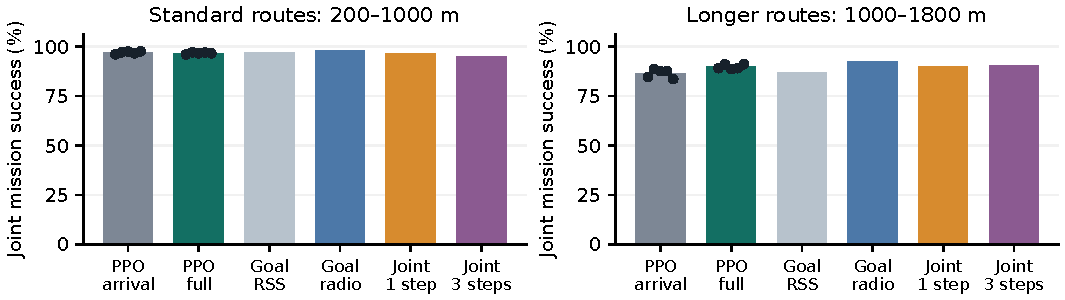
\includegraphics[width=.98\textwidth]{connectivity_success.pdf}
\caption{Strict sampled joint success on fresh routes. Dots show individual
training seeds for learned controllers. Deterministic controllers have one
evaluation per route, not five independent replications.}
\label{fig:success}
\end{figure*}

\section{Results and Interpretation}
\subsection{Strict Joint Completion}
Table~\ref{tab:jointresults} and Fig.~\ref{fig:success} report the frozen results.
The full learned arm achieves \FullStd\% standard and \FullLong\% longer joint
success, compared with \ArrivalStd\% and \ArrivalLong\% for the arrival arm.
The paired standard completion difference is \SuccessDeltaStd\ percentage
points, with 95\% interval [\SuccessLowStd, \SuccessHighStd]. The corresponding
longer difference is \SuccessDeltaLong\ points [\SuccessLowLong, \SuccessHighLong].

Both completion intervals include zero. The prespecified strong joint
improvement claim is therefore not met on either split, despite lower weighted
communication cost. Goal radio has the highest observed completion among the
tested controllers: 98.0\% standard and 92.5\% longer. These results do not
establish a PPO advantage over the simpler reference.

Every reported success has zero observed RSS violations and zero overflow,
as required by the new endpoint. This does not mean every evaluated flight
succeeds. The full arm has \FullFailuresStd\ failed standard evaluations and
\FullFailuresLong\ failed longer evaluations out of 1,000 in each set. Failure
reasons and all per seed outcomes remain in the analysis artifacts.

\subsection{Communication Tradeoffs}
There are \CommonStd\ paired successful standard evaluations and \CommonLong\
longer evaluations for the learned comparison. On those pairs, accumulated
communication cost changes by \CostChangeStd\% and \CostChangeLong\%, respectively.
Table~\ref{tab:pairedradio} shows the individual components and uncertainty.
An improvement in the weighted objective is not equivalent to improvement in
every metric. In particular, the standard mean delay proxy changes by
\DelayChangeStd\%, while handovers change by \HandoverChangeStd\%.

Goal radio improves longer completion over Goal RSS by 5.5 points [1.5, 9.5]
and reduces accumulated cost by 41.0\% on 171 paired successful routes. Three
step planning reduces cost by a further 42.9\% relative to Goal radio on 173
longer pairs, but its completion difference of $-2.0$ points [$-6.5$, 2.5]
does not establish improvement.

On the matched standard routes, the full arm's delay proxy is 4.21 s versus
1.47 s for the arrival arm, while handovers fall from 8.55 to 0.38 per mission.
On matched longer routes, delay is 6.62 s versus 1.83 s. The unweighted
interference difference is inconclusive on both splits. These component
results limit the interpretation of the favorable aggregate cost.

\begin{table*}[!t]\centering
\caption{Full minus arrival on paired successful missions. Differences and 95\% crossed bootstrap intervals. Negative cost, time, delay, interference and handover changes favor full.}
\label{tab:pairedradio}
\begin{tabular}{lrr}\toprule
Metric & Standard difference [95\% interval] & Longer difference [95\% interval]\\\midrule
Accumulated radio cost & $-1.610$ [$ -2.016, -1.230 $] & $-2.393$ [$ -3.317, -1.488 $]\\
Mean radio cost & $-0.060$ [$ -0.075, -0.046 $] & $-0.039$ [$ -0.054, -0.024 $]\\
Arrival time (s) & $-0.195$ [$ -0.267, -0.124 $] & $-0.353$ [$ -0.552, -0.168 $]\\
Delay proxy (s) & $2.738$ [$ 2.030, 3.474 $] & $4.789$ [$ 4.180, 5.397 $]\\
Interference ($\mu$W) & $0.007$ [$ -0.005, 0.018 $] & $-0.002$ [$ -0.012, 0.008 $]\\
Handovers & $-8.165$ [$ -9.226, -7.155 $] & $-19.562$ [$ -21.719, -17.263 $]\\
Mean SINR (dB) & $-1.095$ [$ -1.374, -0.801 $] & $-1.581$ [$ -1.780, -1.393 $]\\
\bottomrule\end{tabular}
\end{table*}

\begin{figure*}[!t]
\centering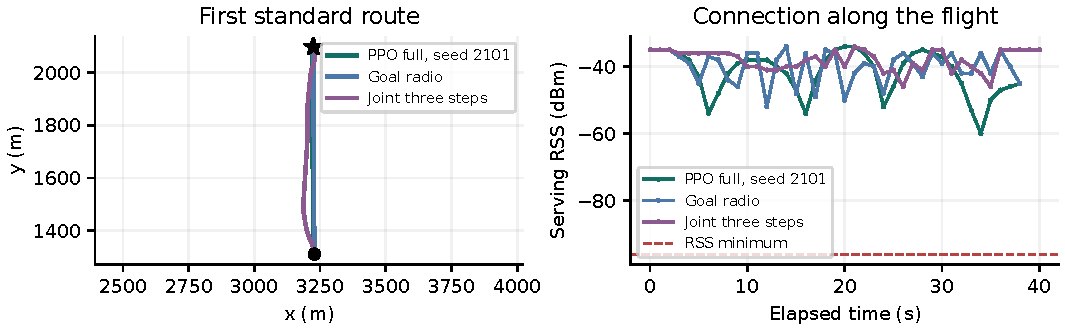
\includegraphics[width=.98\textwidth]{connectivity_example.pdf}
\caption{The first declared standard test route and first full reward training
seed, shown with two model based references. The displayed RSS includes the
initial and terminal sample. This is a fixed example, not a selected typical
route or proof of connectivity between samples.}
\label{fig:example}
\end{figure*}

\subsection{What Is Fixed, and What Remains Open?}
The corrected implementation no longer counts a sampled RSS or buffer
violation as a successful joint flight. Delay, interference and handovers are
active, and admissible RBG choices are explicit. This repairs the earlier
formulation and evaluation omission without making curvature an objective or
guaranteeing success on every feasible mission.

The source's reciprocal tradeoff can tolerate substantial delay and the stated
contract permits a remaining queue at arrival. An application deadline would
require a separately declared requirement, not a retrospective threshold.

Dynamic load, prediction errors, switching interruptions, finer time resolution
and independent maps remain untested. The motion prior and expanded training
range prevent attribution of v2 versus v1 differences solely to reward. Only
the two v2 learned arms isolate the radio cost within their shared architecture.

\section{Reproducibility and Conclusion}
The package retains hashes, routes, ten final and six development checkpoints,
raw outcomes, paired analysis, and Markdown notes with thesis page comparisons.
All 51 tests pass and all 5,600 final evaluations replay exactly. The dataset
and both experiment freezes remain unchanged.

The repair makes communication requirements explicit alongside arrival.
Lower weighted cost coexists with higher delay and uncertain completion
improvement. Remaining failures and surrogate assumptions preclude a claim of
complete physical connectivity or general learned controller superiority.

\begin{thebibliography}{00}
\bibitem{thesis} M. Berm\'udez Granados, ``Deep reinforcement learning based joint
handover and trajectory optimization for 5G connected UAV,'' Master's thesis,
Master's Degree in Artificial Intelligence, UPC, UB, and URV, May 2026.
\url{https://upcommons.upc.edu/entities/publication/a8ce08c2-c238-4145-a5ab-5d39b12c6553}.
\bibitem{ppo} J. Schulman, F. Wolski, P. Dhariwal, A. Radford, and O. Klimov,
``Proximal Policy Optimization Algorithms,'' arXiv:1707.06347, 2017.
\end{thebibliography}
\end{document}
